\chapter{Theoretical foundations}



\section{Molecular fingerprints}

Molecular fingerprint are wiedely used in cheminformatics to represent the structure of molecules for various purposes, such as similarity searching and machine learning in drug discovery.
A plethora of such fariants exist, e.g. Morgan and daylight fingerprints, which extract substructures os the molecule, whereas other descriptors directly incorporate physicochemical properties, e.g. the PaDel-descriptors \cite{Yap.2011}. In the last years, many extensions for improving discernibility of represented models were proposed (see e.g. \cite{Capecchi.2020}).

\subsection{Morgan fingerprint}

One of the most common and successful fingerprints is the Morgan finger print, often also reffered to as ECFP (Extended-Connectivity Fingerprint) \cite{Rogers.2010}.
They are based on the Morgan algorithm, which was first introduced in 1965 \cite{Morgan.1965}. The key idea behind Morgan fingerprints is to represent molecules as a set of circular substructures (atom-centered neighborhoods) rather than paths or subgraphs. 

At the initialization of the algorithm, an atomic representation based on typical features like atom number is created. Each atom in the molecule is assigned an initial identifier based on its atomic properties, such as atomic number, degree (number of bonds), formal charge, and other features. Usually, the features include only very basic properties. Starting at each atom, the algorithm iteratively explores neighboring atoms within a given radius. This circular exploration of the neighbourhood of each atom gives rise to substrctures of increasing size (at radius=1, only the neighbours of the atom are encompassed, for radius=1, also the neighbours of the neighbours and so on).

Using the ECFP-fingerprints based on the Morgan algorithm, one has to be cautious that the number indicates the diameter, i.e. ECFP4 has a radius of 2, ECFP6 of 3.

A hash function is applied to create for each unique substructure a hash value which serves as an almost - except, of course, in the case of collisions - unique identifier. A binary feature vector of fixed length is initialized with zeros and the substructure information is stored by setting for each hash value the according bit in the vector to one, i.e. each entry in the vector tells whether a particular substructure is present or absent.

This process captures structural diversity in a molecule, allowing for comparison between different compounds.

The detrimental occurrence of collisions, i.e. two substructures get the same hash value, can be reduced by increasing the fingerprint size, i.e. the length of the feature vector.

An extension of the Morgan fingerprint does not use bitwise entries, but counts the number of the substructures. In this case, also the frequency of each unique substructure in a molecule is counted and the according value stored in the vector as integer. Of course, in case of molecules composed of many analogous constituents, e.g. fatty chains, this can highly elevate discernibility.


Fig. \ref{fig:morgan_radius} shows the radii 1 and 2 of selects atoms of styrene and fig. \ref{fig:styrene_all_subs_morgan} visualizes all substructures for radius 0 to radius 2 of styrene.




\begin{figure}
    \centering
    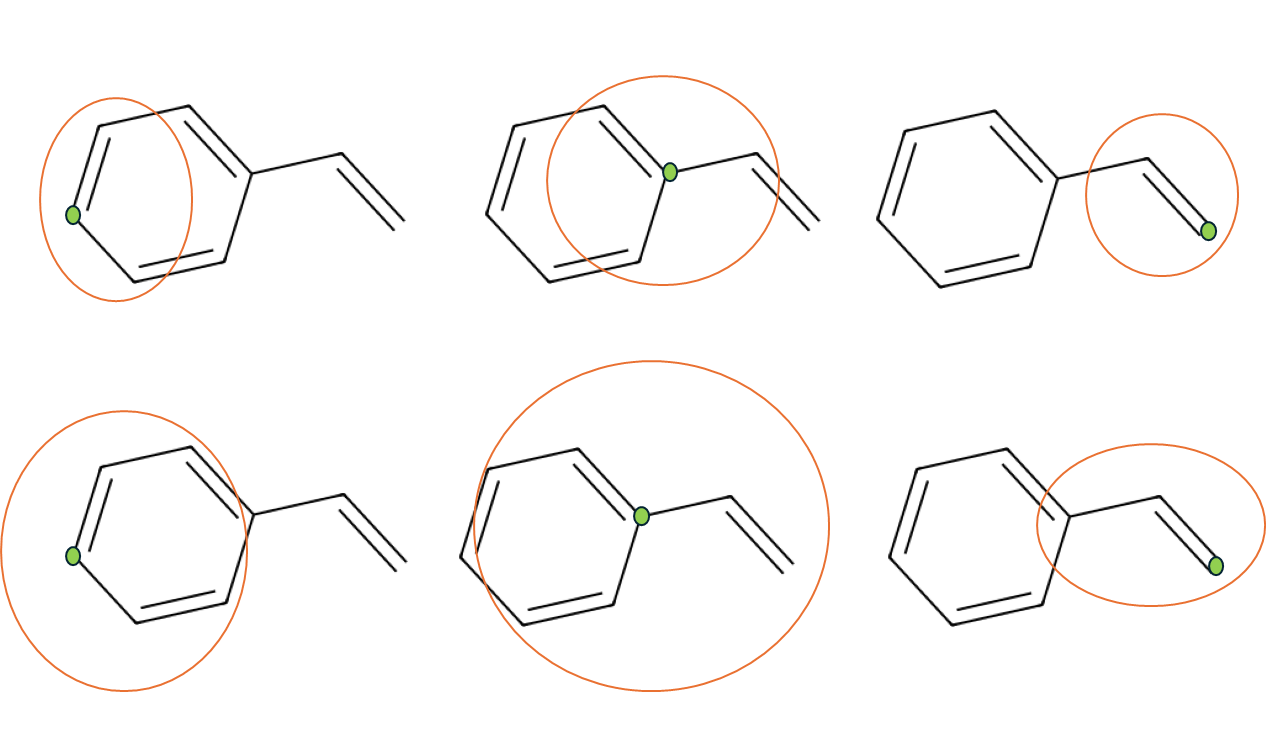
\includegraphics[width=1\linewidth]{morgan_radius.png}
    \caption{radii of selected atoms up to radius 2 for styrene}
    \label{fig:morgan_radius}
\end{figure}


\begin{figure}
    \centering
    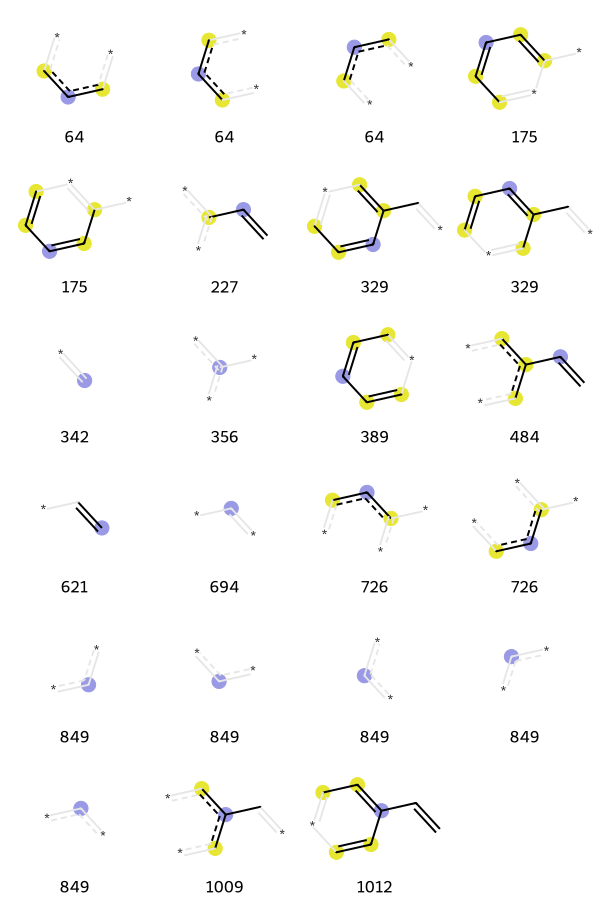
\includegraphics[width=1\linewidth]{styrene_all_subs_morgan.png}
    \caption{all substructures of styrene up to radius 2}
    \label{fig:styrene_all_subs_morgan}
\end{figure}

\begin{figure}
    \centering
    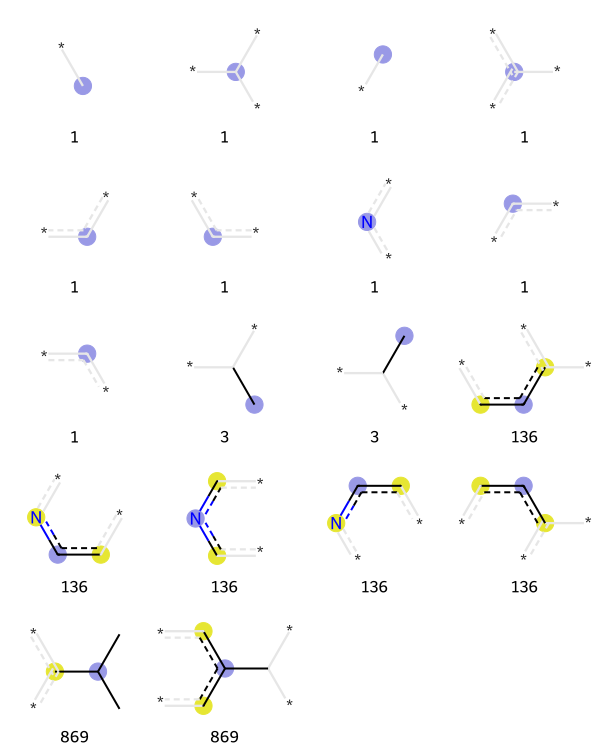
\includegraphics[width=1\linewidth]{substructures_radius1_only_topology.png}
    \caption{Enter Caption}
    \label{fig:substructures_radius1_only_topology}
\end{figure}


\section{Graph Neural Networks}

Graph Neural Networks work on graph data; they can be seen as generalizations of convolutional neural networks (CNNs).

Unlike traditional fingerprints, GNNs treat molecules as graphs, where atoms are nodes and bonds are edges. This structure allows GNNs to directly process the molecular graph and learn more flexible, task-specific representations via message-passing mechanisms. Given that GNNs operate on graph data, they are naturally suited for capturing the intricate connectivity patterns of molecules, which are central to their properties.

They can be applied for different purposes, like node (for individual nodes of the graph, labels or values are predicted)    and graph classification (for the whole graph, a label or value is predicted) as well as link prediction (prediction of the likelihood that an edge exists between specific nodes). In the context of molecular property prediction, one usually deals with graph classification problems, e.g. the label (indicating toxicity, inhibitory activity, etc.) or a value (solubility, lipophilicity, etc.) for the graph which represents a specific molecular compound is determined.

In the following experiments, in particular Graph Convolutional Networks (GCNs) and Graph Isomorphism Networks (GINs) were considered.

It should be noted that there is a much greater variety of GNNs. Some of them, like GATs, yield impressive performance in some tasks.

Most Graph Neural Networks rely on message passing. Different specific architectures are termed MPNN, the central property of the general framework is that a message passing and a readout step are involved. In the context of molecular property prediction, this scheme was introduced in \cite{Gilmer.05.04.2017}.

In the message passing step, each node of the graph passes its feature information to its neighbors and aggregates the information received from them. This process is repeated across multiple layers, allowing each node to gather information from increasingly distant nodes in the graph.

After the graph layer operations, the output has to be arranged in such a way that it can be used for the final prediction, done in the readout step.
Common read-out functions are max and mean; for graph classification and in molecular property prediction, it has turned out that sum is most powerful.

This is usually done using a dense neural network (DNN). (In principle, also a different classifier, e.g. SVM or gradient boost algorithms, could be used; however, for such a set-up backpropagation is probably not feasible. One would have to train the GNN with a simple output layer and after training use the embedding of the GNN as input for the classifier.)

In contrast to Morgan fingerprints, which either provide binary or integer vectors, the GNN architectures usually output a real-valued vector. (Some proposals for creating a representation more similar are proposed below.)

In principle, all GNN architectures suitable for Graph classification can be used for molecular property prediction; however, also some variants like the Attentive Fingerprint are explicitly modeled for this task.

\subsubsection{GCNs}

One of the most commonly used GNN architectures is the Graph Convolutional Neural Network. It can be seen as a generalization of CNNs; whereas the latter can only process input of fixed size, GCNs act directly on the graph representation. As for most graph-based representations, the graph information consists of the adjacency matrix (which in the case of molecule property prediction usually encodes the bonds between atoms) and a feature matrix (which encompasses the physicochemical features of the atoms, e.g. atom type).

Usually, multiple graph convolution layers are stacked. Each layer enriches the represention of a specific node by exploring larger neighbourhoods of the graph. In particular, the first layer aggregates features from the direct neighbours. After this layer, information of the neighbours is stored in each feature representation, so in the next layer also information about the neighbours of the neighbours is incorporated etc.

In the central graph convolution step, neighborhood aggregation is performed: 
\begin{equation}
H^{(l+1)} = \sigma\left(\tilde{D}^{-1/2} \tilde{A} \tilde{D}^{-1/2} H^{(l)} W^{(l)}\right)
\end{equation}


, where W denotes the learnable weight matrix, A the adjacency matrix and D the diagonal degree matrix. \begin{math}\sigma\end{math} corresponds to an activation function, e.g. the often used Rectified Linear Unit activation function (ReLU).


One disadvantage of GCNs is, that they use a mean-based aggregation and this function is not injective. This means that different graphs can lead to the same graph embedding and the network cannot distinguish between the two graphs anymore. One example is visualized in Figure 3 below. Assuming the node and edge properties are identical, GCNs could create the same hidden embedding for these two graphs.

For molecular property prediction, the severity of these limitations relies on several factors (see below); for instance, the occurrence of different, but undistinguishable graphs crucially depends on the used features.

\subsubsection{GINs}

The aggregation function here is a sum.

\cite{Xu.01.10.2018}
GINs (Graph Isomorphism networks) excel in distinguishing different graph structures. It can be shown that they are as expressive as the Weisfeiler Leman algorithm for detecting graph ismorphisms. 
The WL test is determines whether two graphs are isomorphic, i.e. structurally identical, regardless of their labeling.
Thus, if the Weisfeiler Leman algorithm is able to distinguish two graphs, they can also be distinguished by GIN networks. \cite{}


The aggregation function in a Graph Isomorphism Network (GIN) is defined as:

\[
h_v^{(k+1)} = \text{MLP} \left( (1 + \epsilon) \cdot h_v^{(k)} + \sum_{u \in \mathcal{N}(v)} h_u^{(k)} \right)
\]

Where:
\begin{itemize}
    \item \( h_v^{(k)} \) is the feature vector of node \( v \) at layer \( k \),
    \item \( \mathcal{N}(v) \) denotes the set of neighbors of node \( v \),
    \item \( \epsilon \) is a learnable (or fixed) scalar parameter,
    \item \(\text{MLP}\) represents a multi-layer perceptron applied to the aggregated features.
\end{itemize}

The feature aggregation is computed by summing over all neighbours of the node (in principle, also a different aggregation function can be applied, but the sum-function works best for distinguishing graphs).

\( \epsilon \) determines how strongly the node's own features influence the aggregation. It can be implemented as a learnable parameter or set to a fixed value. (Obviously, setting \( \epsilon = 1\), one can eradicate the own features.) 
Similarly to GCN, multiple layers can be stacked to explore the more distant neighbourhood of the graph because at each layer information from the more distant neighours is propagated by feature aggregation.



\subsubsection{GINE}

GINE is an extension of GIN; in contrast to the former, GINE also uses bond information\cite{Hu.29.05.2019}.
This process involves a summation of bond and edge features which requires that the dimensionality of both types of features is identical. (This can be easily attained by adding a preceding linear layer to one type of features with an output layer identical in size to the feature dimensionality of the other feature type, i.e. either for the node or the edges features an embedding with the dimension of the other feature type is created.)



The node update rule for the Graph Isomorphism Network with Edge Features (GINE) is given by:

\[
h_v^{(k+1)} = \text{MLP}^{(k)} \left( (1 + \epsilon^{(k)}) \cdot h_v^{(k)} + \sum_{u \in \mathcal{N}(v)} \text{ReLU} \left( h_u^{(k)} + e_{uv} \right) \right)
\]

Where:
\begin{itemize}
    \item \( h_v^{(k)} \) is the feature vector of node \( v \) at layer \( k \),
    \item \( h_u^{(k)} \) is the feature vector of a neighboring node \( u \) at layer \( k \),
    \item \( \mathcal{N}(v) \) is the set of neighbors of node \( v \),
    \item \( e_{uv} \) is the feature vector of the edge between nodes \( u \) and \( v \),
    \item \( \epsilon^{(k)} \) is a learnable or fixed scalar parameter for layer \( k \),
    \item \(\text{MLP}^{(k)}\) is a multi-layer perceptron for layer \( k \)
\end{itemize}


\subsubsection{GAT}

Graph Attention Networks incorporate information about the neighbourhood of each node by applying a local attention mechanism \cite{Velickovic.30.10.2017}.


Attention scores are computed by introducing a learnable weight vector, e.g.:

e_{ij} = \text{LeakyReLU}\left( \mathbf{a}^\top \left[ \mathbf{W} \mathbf{h}_i \parallel \mathbf{W} \mathbf{h}_j \right] \right)

To obtain normalized attention weights, a softmax function can be applied:



\alpha_{ij} = \text{softmax}_j(e_{ij}) = \frac{\exp(e_{ij})}{\sum_{k \in \mathcal{N}(i)} \exp(e_{ik})}

This attention mechanism should allow to capture long-range dependencies (i.e. influence from more distant nodes) and focus on the most relevant interactions.
The aggregation of the feature vectors of a specific node and its neighbours is weighted by the attention weights.

Graph Attention Networks (GATs) integrate information from the neighborhood of each node by employing an attention mechanism, as introduced in \cite{Velickovic.30.10.2017}. The attention mechanism begins by computing attention scores between node pairs. These scores are determined using a learnable weight vector:

\[
e_{ij} = \text{LeakyReLU}\left( \mathbf{a}^\top \left[ \mathbf{W} \mathbf{h}_i \parallel \mathbf{W} \mathbf{h}_j \right] \right)
\]

To normalize these attention scores, a softmax function is applied, producing attention weights:

\[
\alpha_{ij} = \text{softmax}_j(e_{ij}) = \frac{\exp(e_{ij})}{\sum_{k \in \mathcal{N}(i)} \exp(e_{ik})}
\]

This attention mechanism allows GATs to capture long-range dependencies (i.e., interactions between distant nodes) and to focus on the most relevant connections. The feature vectors of a node and its neighbors are then aggregated, weighted by the computed attention weights:

\[
\mathbf{h}_i^{\text{(new)}} = \sigma \left( \sum_{j \in \mathcal{N}(i)} \alpha_{ij} \mathbf{W} \mathbf{h}_j \right)
\]

In the multi-head attention setting, the updated node feature representation becomes:

\[
\mathbf{h}_i^{\text{(new)}} = \sigma \left( \frac{1}{K} \sum_{k=1}^{K} \sum_{j \in \mathcal{N}(i)} \alpha_{ij}^{(k)} \mathbf{W}^{(k)} \mathbf{h}_j \right)
\]

Here, \( \mathbf{h}_i \in \mathbb{R}^F \) represents the initial feature vector of node \(i\), and \(\mathbf{W}\) denotes a learnable weight matrix. The aggregation process results in the node's new feature representation, \( \mathbf{h}_i^{\text{(new)}} \), after applying the activation function \( \sigma \).

Finally, the loss function used for optimization in GATs is typically defined as:

\[
\mathcal{L} = - \sum_{i \in \mathcal{V}} \sum_{c=1}^{C} y_{ic} \log \hat{y}_{ic}
\]

Different variants exist, e.g. a revised version of the original GAT layer, introduced in \cite{Brody.30.05.2021b}, further improves its performance by addressing some of its limitations.






\subsubsection{Neural Fingerprint}



The Neural Fingerprint, introduced in \cite{Duvenaud.30.09.2015}, was the first graph neural network architecture developed for molecular property prediction. In the experiments presented in \cite{Duvenaud.30.09.2015}, Neural Fingerprints outperformed circular fingerprints, particularly when paired with a linear neural network classification layer on all test datasets. However, the comparisons shown were limited to binary Morgan fingerprints.

A distinctive feature of the Neural Fingerprint is its use of degree-dependent weight matrices. This means that nodes with different degrees are updated using distinct weight matrices. The update rule for node features, as implemented in PyTorch Geometric (see the next chapter), is given by:

\begin{equation}
\mathbf{x}_i' = \mathbf{W}_1^{(\text{deg}(i))} \mathbf{x}_i + \mathbf{W}_2^{(\text{deg}(i))} \sum_{j \in \mathcal{N}(i)} \mathbf{x}_j
\end{equation}



Here, \(\mathbf{x}_i\) represents the feature vector of node \(i\), and \(\text{deg}(i)\) is its degree. The updated features are passed through a sigmoid activation function. Finally, the output is multiplied by learned output weights, and a softmax function is applied to generate the final fingerprint vector. This vector is intially initialized as a zero vector (similar to Morgan fingerprints), and at each layer the contribution from each atom is added to the vector according to the softmax function output.

The Neural Fingerprint shares some conceptual similarities with Graph Isomorphism Networks (GINs). Both architectures aggregate information from the neighbors of a specific node and update the node features accordingly. However, unlike GINs, which use a multi-layer perceptron (MLP) and summation-based aggregation, the Neural Fingerprint uses degree-dependent weight matrices and applies a fixed sigmoid activation function.
In contrast to the processing the sum of the neighbour nodes and self-node update within the MLP, in case of the Neural Fingerprint weight matrices are learnt and a fixed activation function (sigmoid function) is applied.


\subsubsection{Attentive Fingerprint}

The Attentive Fingerprint was proposed in \cite{Xiong.2020} as an extension of the Neural Fingerprint leveraging attention.
In contrast to GCNs and GINs, it also incorporates edge information directly. It extends the idea of the Neural Fingerprint with an attention mechanism similar to that used in GAT. In fact, GAT layers are part of the attentive fingerprint, i.e. it is a specific implementation of this architecture.
The update step in the Attentive Fingerprint shares similarities with the approach used in GCNs, but it integrates attention weights to emphasize the most relevant interactions. These attention weights are computed using a combination of GRU cells and GAT convolutions. 

The implementation provided via PyTorch Geometric uses the original GAT formulation for these convolutions.



\begin{table}[h!]
\centering
\begin{tabular}{|>{\raggedright\arraybackslash}p{3.5cm}|>{\centering\arraybackslash}p{1cm}|>{\raggedright\arraybackslash}p{7cm}|}
\hline
\textbf{Atom Feature} & \textbf{Size} & \textbf{Description} \\
\hline
Atom symbol & 16 & [B, C, N, O, F, Si, P, S, Cl, As, Se, Br, Te, I, At, metal] (one-hot) \\
\hline
Degree & 6 & Number of covalent bonds [0,1,2,3,4,5] (one-hot) \\
\hline
Formal charge & 1 & Electrical charge (integer) \\
\hline
Radical electrons & 1 & Number of radical electrons (integer) \\
\hline
Hybridization & 6 & [sp, sp$^2$, sp$^3$, sp$^3$d, sp$^3$d$^2$, other] (one-hot) \\
\hline
Aromaticity & 1 & Whether the atom is part of an aromatic system [0/1] (one-hot) \\
\hline
Hydrogens & 5 & Number of connected hydrogens [0,1,2,3,4] (one-hot) \\
\hline
Chirality & 1 & Whether the atom is a chiral center [0/1] (one-hot) \\
\hline
Chirality type & 2 & [R, S] (one-hot) \\
\hline
\textbf{Bond Feature} & \textbf{Size} & \textbf{Description} \\
\hline
Bond type & 4 & [single, double, triple, aromatic] (one-hot) \\
\hline
Conjugation & 1 & Whether the bond is conjugated [0/1] (one-hot) \\
\hline
Ring & 1 & Whether the bond is in a ring [0/1] (one-hot) \\
\hline
Stereo & 4 & [StereoNone, StereoAny, StereoZ, StereoE] (one-hot) \\
\hline
\end{tabular}
\caption{Atom and Bond Features Table}
\label{tab:features}
\end{table}


\subsubsection{Higher-order and subgraph GNNs}

Alternatively to the stacking of multiple GNN layers, the incorporation of global information and thus increased expressivity can also be attained via Higher-order GNNs which were propsed in \cite{Morris.04.10.2018}

The concept of Subgraph GNNs is tightly related to Higher-order GNNs.

A recently published type of Subgraph GNN which resembles fingerprints is the Nested GNN \cite{Zhang.2021}. 

However, rooted subtrees have limited expressiveness for representing non-tree graphs. To overcome this, Nested Graph Neural Networks (NGNNs) are proposed, which use rooted subgraphs instead of subtrees.

This approach improves distinguishability between graphs; for instance, many rr-regular graphs, which are not distinguishable by the 1-WL test, have distinct NGNN representations nonetheless.

NGNN works by extracting local subgraphs around each node, applying a base GNN to learn subgraph representations, and pooling these into a whole-graph representation. 


Since all subgraphs are copied to the GPU memory, this approach is - depending, of course, on the available resources - only feasible for rather small graphs (as it is typical for molecular graphs).

Similarly, for Nested GNNs high variance was reported in \cite{Zhang.2021}. They trained for a fixed number of epochs. In addition to the final model, every 10 epochs a checkpoint was created, and the average ensemble performance was also reported.

Each subgraph up to a specific radius is evaluated; as base GNN various architectures, e.g. GCN and GIN, can be used.
In \cite{Zhang.2021}, this architecture was tested on the QM9 dataset and the HIV and PCBA datasets.



\subsection{Combination of fingerprint and GNN information}

Meanwhile, it was also explored whether the combination of molecular fingerprint and graph-based representations can improve predictive power. A simple approach computes both separately and passes both outputs to a final classifier (e.g. a dense neural network layer, but also a different architecture depending on the task would be possible).

In \cite{Zhang.2024}, several different fingerprints were computed and a feature selection module created a reduced version by maximizing relevance and minimizing redundancy. 

Similar to \cite{Zhang.2024}, fingerprint and GNN information was also combined.


In \cite{Liu.2025}, a model called fingerprint-enhanced hierarchical graph neural network (FH-GNN) is proposed.
On eight benchmark datasets from MoleculeNet, it outperformed many baseline models and competitors.  


In many cases, results are ambiguous. For example, the complex graph-based architecture proposed in \cite{Yang.2019} achieved superior results on some datasets, but on other it performed equal or even worse than a Random Fores classifier applied on fixed molecular fingerprint representations.

Another approach uses fragmentation methods like BRICS to obtain processable, chemically or archaeologically meaningful substructures of a molecule \cite{Degen.2008,Jinsong.2024,ZhangBRICS.2024,Liu.2017,Diao.2023}.


\subsection{More complex architectures for molecular property predictions}


In \cite{Alon.09.06.2020}, an additional fully adjacent layer (in which all nodes are connected) was applied in order to attenuate bottleneck effects.

For example, \cite{Liu.2025} and \cite{Zang.2023} use the BRICS algorithm to create fragments for a hierarchical molecular graph.


or hierarchical molecular graph neural networks (HimGNN) \cite{Han.2023}, which applies a Transformer architecture to fuse atom- and molecular motif-based graphs.

Hyper-Mol creates a molecular graph representation based on the preceding extraction of ECFP fingerprints \cite{Cui.2023}.

A message passing algorithm using bond information (instead of the usual node based message passing), termed directed MPNN (D-MPNN), was proposed in \cite{Yang.2019}. This message passing scheme is directed in such a way that the messages at the current step are not influenced by the message in the reverse direction from the previous step, attenuating the problem of tottering.


Bitwise and Count fingerprints were also used as baseline in \cite{Yang.2019}. For some datasets, similarly large differences were found, but not in all; a plausible explanation is different, and possibly insufficient, hyperparameter optimization. Indeed, it is noted in \cite{Yang.2019}, that all architectures (baseline as well as the newly proposed D-MPNN) are applied with unspecified default parameters (making a fair comparison virtually impossible, see results and discussion section).

Another approach features data augmentation and contrastive learning \cite{Wang.2022} .Motif-driven contrastive learning is also applied in \cite{Zhang.2024b} and multiple molecular graph representations of different granularity are combined in \cite{Kengkanna.2024}.

Another self-supervised pre-training scheme was proposed in \cite{Wan.2025}. In \cite{Wan.2025}, also performance in the presence of activity cliffs was studied in more detail. Similarly DGCL, uses a similar combination of two GNNs (GIN and GAT) and additionally incorporates fingerprint information \cite{Jiang.2024}. The version with both GNNs was compared to architectures consisting of ECFPs combined with pre-trained GIN and GAT layers. These combinations improved performance on some datasets (however, unfortunately, the ECFP baseline was not checked, so it is difficult to fully assess the performance gain).

Other graph-based approaches apply self-supervised learning. For instance, GROVER (Graph Representation frOm self-superVised mEssage passing tRansformer), a transformer-based framework with 100 million parameters, which was pre-trained on 10 million unlabelled molecules \cite{Rong.2020}, is widely used.

Similarly, MolBERT is a BERT model pre-trained on four million unlabeled compounds which can be used for  molecular property prediction tasks \cite{Li.2021}. Interestingly, as shown in the discussion below in more detail, even these large models do not persistently outperform simpler GNN architectures or even ML classifier acting on Morgan fingerprints.

\section{Activity cliffs}

Recently, in the context of QSAR, the role of activity cliffs is intensively discussed. Such activity cliffs consist of molecules which are structurally very similar, but feature highly different molecular properties.

This implies that the structural differences cause big biological differences.\cite{Stumpfe.2019} It is crucial to not confuse them with outliers \cite{Maggiora.2006}.

In particular, it is astonishing that molecular fingerprints outperform GNNs especially in ‘difficult’ tasks which should be more suited for the latter, e.g. in activity cliff prediction.

Also \cite{Jiang.2021} rightly mentions that these evaluations are often rather biased against the classical fingerprints. For example, for ECFP only Random Forests and Support Vector Machines are tried as classifiers, but newer, more complex and potentially superior ML classifiers, e.g. gradient-boosting techniques like LightGBM, are not included in the benchmark. In many cases, also hyperparameter optimization can lead to performance distortions which are wrongly interpreted as essential differences between the architectures. 


\section{Previous work}

Similarly, in \cite{Jiang.2021} classical fingerprints in combination with a DNN or a classical ML algorithm (e.g. support vector machines or random forests) outperformed graph-based models in most tasks. Only for some larger and multi-task datasets graph representations yield better performance than the descriptor-based models, implying that data availability is critical. (However, studies systematically evaluating the impact of additional data on specific datasets are largely missing.)
The graph models investigated in \cite{Jiang.2021} were GCNs, attentive FP and a MPNN model; GIN was not applied.

Graph-based models show better performance only on larger dataset.
SVM generally achieves the best predictions for the regression tasks. Both RF and XGBoost can achieve reliable predictions for the classification tasks, and some of the graph-based models, such as Attentive FP and GCN, can yield outstanding performance for a fraction of larger or multi-task datasets. In terms of computational cost, XGBoost and RF are the two most efficient algorithms and only need a few seconds to train a model even for a large dataset. The model interpretations by the SHAP method can effectively explore the established domain knowledge for the descriptor-based models.
 
On the HIV dataset, it was shown that different classifiers yield different profiles.

In \cite{Dablander.2023}, the performance of ECFPs and other descriptors is compared to GINs on several binding affinity data sets with a focus on activity-cliff prediction. The authors state that activity cliffs seem to be a major problem for accurate predictions and, on average, graph-based representation cannot handle them more efficient than the simpler fingerprints. 

Similarly, \cite{Stepisnik.2021} state that deep learning approaches do not yield better performance compared to classical fingerprints in spite of their much higher computational cost.

In the same vein, \cite{Deng.2023} stresses the importance of activity cliffs.

Moreover, in some cases, circular fingerprints coupled with a classical ML method, e.g. support vector machines, outperformed a DNN version. Again, this was the case in a study focusing on activity cliffs using CHembl.

However, it should be noted that most of these studies show serious flaws or gaps (which will become even more obvious regarding the results of this investigation).

In \cite{Jiang.2021}, the models were evaluated on 50 random splits. Although one could argue that the comparatively high number of runs cover a wide range of possible combinations, this procedure does not substitute for other splits.
Moreover, hyperparameter optimization only processed a small list of possible values for parameters like the hidden channel size within a limited range, possibly reasonable parameter combinations were missing; for continuous variables like the learning rate only a few possible values were assigned. Furthermore, techniques like normalization layers were not considered (dropout was only a parameter for the final prediction layer). 


However, a meta-analysis of the results is hardly possible because often the indication of crucial parameters is missing. For instance, it is not always clear which atom and node features have been used (it can be assumed that likely the default featurizer of the used GNN framework was applied; since many frameworks have specialized featurizers for specific architectures, it is even more difficult to decide). Hence, it could be necessary to evaluate the impact of such factors.

In the same vein, the Attentive FP, i.e. the application of GAT to molecular property prediction, proposed in Xiong et al. 2020 showed superior performance in almost all tasks from MoleculeNet. However, only three runs were performed and for regression tasks like ESOL solely random splits were applied. Furthermore, as in \cite{Duvenaud.30.09.2015}, it seems that the ECFP used only bitwise features which leads to much worse performance of the fingerprint.

For the regression tasks, mostly the random split is used. Furthermore, for the classification tasks of MoleculeNet, except for the MUV-dataset, usually ROC-AUC is used as metric, although all datasets are rather imbalanced (e.g. in \cite{Zhang.2024}). In particular, it should be noted that for scaffold splits the imbalance can be much higher than for the complete dataset, hence leading to a potentially misleading ROC-AUC.

It is also problematic that sometimes error estimates (e.g. in \cite{Zhang.2024}) are missing, which makes the ranking of the classifiers in case of small differences (or possibly high inter-run variances) impossible.

Similarly, in \cite{vanTilborg.2022}, all models were trained for 300 epochs and the early stopping patience was set to ten epochs, which arguably is a very low number in this setting (especially given the fact that most datasets are not very big), possibly excluding good solutions.

High inter-run variance as well as small parameter deviations probably explain that results often cannot be replicated.
For instance, in \cite{Zhang.2024}, a new hybrid fingerprint-GNN approach is presented and compared against other algorithms like Attentive FP. 
In the original publication, for ESOL, FreeSolv and lipophilicity, values of 0.503, 0.736 and 0.578 were reported; the evaluation of Zhang provided 0.587, 1.091 and 0.553.

These issues are extensively discussed in \cite{Wallach.2018}

Furthermore, the inference from low p-values (without accompanying effect sizes) that there is a significant effect is correctly criticized given the fact that for increasing sample size (which can be arbitrarily increased by evaluating a higher number of test splits) p-values get arbitrarily low. \cite{Robinson.2020} 

It should be noted that protein-ligand and ligand-ligand interaction tasks often provide spurious results \cite{Volkov.2022}.
Even when it is unlikely due to these problems that one gets results sufficiently reliable for practical application, the comparison between circular fingerprints and GNNs could also be insightful in this case.



\section{Potential Pitfalls and Limitations}

Over-fitting, over-smoothing, and over-squashing represent significant challenges to the performance of Graph Neural Networks (GNNs) \cite{JunXia.2023}.

Fundamental limits of expressivity, i.e. there are graphs which cannot be distinguished by GNNs working with the message passing paradigm, have also to be taken into account. However, since in most molecular property prediction tasks the central goal is not to have a unique mapping of each molecule, but a representation which allows an accurate prediction of the objective value. (In principle, for a binary classification task it would be sufficient to map all input graphs to two different output vectors.)


Over-smoothing occurs predominantly in models with stacked graph layers. After several layers, node embeddings tend to converge to similar values, which diminishes the ability of the model to differentiate between nodes and often leads to degraded performance. This is highly problematic in the context of molecular property prediction.


Over-fitting is particularly challenging in molecular property prediction tasks. This issue stems from two main factors: Firstly, there is often a limited availability of training examples, and, exacerbating the problem, data is often highly imbalanced. Secondly, one has to consider substantial differences between training and test examples, which make over-fitting to the training data especially detrimental.

Over-squashing arises when the graph topology creates a bottleneck for message propagation, distorting the flow of information. While this phenomenon can severely affect certain graph types, it is generally less problematic for smaller graphs, such as those commonly used in molecular applications.

\cite{CortesCiriano.2019} used Morgan Fingerprints with a comparatively small size (128) as input for DNN and RF ensembles, reporting that larger fingerprint sizes did only marginally improve results. In this publication, another technique called snapshot ensemble learning is introduced \cite{CortesCiriano.2019}. The training process is divided into cycles and after each converged cycle the learning rate is set back to its original value.

Furthermore, in the creation of datasets like HIV and the toxicity-related ones, a threshold for obtaining binary classification labels was applied. This allows that there are very similar molecules in terms of the original value, which are artificially separated into two different groups due to the threshold.




In \cite{TranNguyen.2020}, where the LIT-PCBA dataset is presented, these problems are well summarized:
'Intriguingly, DNNs trained with rigorous crossvalidation procedures on simple ligand descriptors were almost as accurate as those trained on protein−ligand attributes, evidencing that deep learning did not learn anything about the physics of protein−ligand interactions. Strikingly, the literature is full of overoptimistic reports describing machine learning models with near perfect performances on the above described data sets, although true VS practitioners have known for a long time that such an accuracy level does not mirror the proportion of experimentally confirmed hits in real prospective VS experiments.' \cite{TranNguyen.2020}


Moreover, most GNN architectures have been introduced with very specific parameters. For instance, in the AttentiveFP paper it is not taken into account that also the selection of node and edge features (which differs strongly from other set-ups) could be responsible for the performance gain (and not the newly proposed architecture itself).